\documentclass[a4paper,12pt]{article}
\usepackage[english]{babel}
\usepackage[utf8]{inputenc}

\usepackage[top=2.5cm, bottom=2.5cm, left=2cm, right=2cm]{geometry}

\usepackage{datetime}
\newdateformat{monthyeardate}{%
  \monthname[\THEMONTH], \THEYEAR}

\usepackage{subcaption}

% Math packages
\usepackage{mathtools}
\usepackage{amsmath}
\usepackage{amsfonts}
\usepackage{amssymb}

\usepackage{enumitem}
\usepackage{algorithm}
\usepackage{algpseudocode}

\usepackage{listings}

\usepackage{makecell}

\usepackage[hidelinks]{hyperref}

\title{Mobile and Social Sensing Systems}
\author{Francesco Barbarulo, Giovan Battista Rolandi}
\date{\monthyeardate\today}

\begin{document}
\pagenumbering{roman}

\maketitle
\abstract{The aim of these notes is to give some pills of every argument for the oral test. We have assumed that the reader has attended the lessons because these notes, by themselves, are not sufficient to have a global and profound knowledge.

We wish you good luck!}

\tableofcontents

\newpage

\pagenumbering{arabic}

\section{Introduction}
\subsection{Mobility}
\begin{itemize}
    \item \textbf{Physical}: hardware actually changes its physical position;
    \item \textbf{Logical}: applications and data may need to be moved for design reasons.
\end{itemize}

Mobile computing relys on the ability to use devices \textit{non-physically connected} and \textit{context-aware}. These devices must keep computinal and communicaiton capabilities paying attention to energy comsumption because of their battery-powered nature.

\section{Localization systems}
Localization systems consist of two main blocks:
\begin{enumerate}[label=(\roman*)]
	\item Set of deployed nodes with different \textit{states}:
		\begin{itemize}
		 	\item \textbf{beacon} (\textit{landmarks} or \textit{anchors}): already know their locations through a manual configuration or through GPS reading;
		  	\item \textbf{unknown} (\textit{targets}): do not have any information about their geographic locations;
		  	\item \textbf{settled}: targets nodes that has determined or estimated their locations.
		\end{itemize}
	\item Localization algorithm:
		\begin{itemize}
			\item GPS not longer used in CPS for cost and energy constraints;
			\item \textbf{GPS-free} techniques exploit the sensing and the wireless communication capabilities of CPS components.
		\end{itemize}
\end{enumerate}

\subsection{Topology}
The topology of a localization algorithm refers to \textit{where} and \textit{how} the location of a given node is calculated:

\begin{itemize}
	\item \textbf{Centralized localizaiton}: a central device estimates the location of unknown nodes based on the signal measurements forwarded by anchors;
	\item \textbf{Localized localization}: each object estimates its location using the collected signal measurements and location information of the anchor nodes in its neighbourhood.
\end{itemize}

We can distinguish four different system topologies for localization systems, as shown in Figure~\ref{fig:topology}.
\begin{figure}
	\centering
  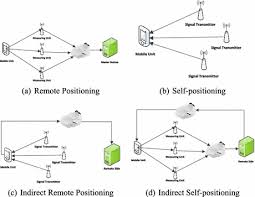
\includegraphics[width=0.6\textwidth]{img/topology}
  \caption{\label{fig:topology}Taxonomy of localization systems topology}
\end{figure}

\subsection{Coordinate System}
\begin{itemize}
  \item \textbf{Physical}: locations are represented as a point in a 2D/3D coordinate system;
  \item \textbf{Symbolic}: locations are expressed as logical positions’ information;
  \item \textbf{Absolute}: locations are expressed as unique coordinate values making reference to \textit{anchor} nodes that know their positions;
  \item \textbf{Relative}: locations are determined relatively to other nodes with no reference to absolute anchors.
\end{itemize}

\subsection{Communication paradigm}
\begin{itemize}
  \item \textbf{Non-cooperative}: the communication is restricted between unknown nodes and anchors (\textit{high density} of anchors or \textit{long-range anchor transmissions} are needed);
  \item \textbf{Cooperative}: allows communication between unknown nodes (more \textit{processing} is required);
  \item \textbf{Opportunistic}: exploits interactions between nodes that occasionally pass each other in their proximity (efficient \textit{node discovery} and \textit{data exchange}).
\end{itemize}

\subsection{Performance metrics}
\begin{itemize}
  \item \textbf{Accuracy}: mean (Euclidean) distance error between the estimated location and the true location;
  \item \textbf{Precision}: variation over many algorithm trials, CDF of distance error;
  \item \textbf{Complexity}: hardware and/or software;
  \item \textbf{Robustness}: behavior under unwanted conditions;
  \item \textbf{Scalability}: geographical and density;
  \item \textbf{Cost}
\end{itemize}

\subsection{Category}
The catogery of the localization technique pertains to how the location of a node is calculated depending on whether they are based on distance measurement or not. The two main categories are: \textit{range-based} and \textit{range-free}. 

Note that all the presented techniques are classified as \textit{anchor-based} schemes, assuming the existence of nodes with known positions.

\subsubsection{Range-based}
Range-based (or distance-based) techniques rely on the computation of distances between the target node and the anchor nodes to infer the position of a target node using \textit{lateration} techniques.

Location discovery consists of two phases:
\begin{enumerate}
  \item \textbf{Ranging phase} (or measuring distance): each node estimates its distance or angle from neighbors based on information contained in \textit{beacon} messages.
  The main three distance measuring methods are: 

  \begin{enumerate}[label=(\roman*)]
    \item \textit{Received Signal Strength (RSS)} estimates the distance from some set of neighbors using the attenuation of emitted signal strength. In free space, the RSS varies as the inverse square of the distance $d$ between the transmitter and the receiver:

    \begin{equation}
    P_r(d) = \frac{P_t G_t G_r \lambda^2}{(4\pi)^2 d^2}
    \end{equation}

    where $ P_r $ and $ P_t $ are respectively the reception and transmission power, $ G $ is the antenna gain, $ \lambda $ is constant and $ d $ is the distance between transmitter and receiver. Unfortunately, RSS is unreliable as it gets affected by the random multi-path effect.

    The parameters employed in these models are \textit{site-specific} and an empirical model is derived by obtaining a least square fit for each power level:

    \begin{equation}
    P_{RSSI} = \frac{X}{d^n}
    \end{equation}

    \item \textit{Time of Arrival} consists in calculating the one way propagation time of radio signals (RF) between two \textbf{synchronized} nodes. This time is proportional to the distance between transreceivers and is given by Eq.~\ref{eq:toa}:

    \begin{equation}
    d = c_r \times (t_1 - t_0)
    \label{eq:toa}
    \end{equation}

    This method of RF signals is usually inappropriate for WSNs because of short distances and inaccurate time synchronization of sensor nodes.

    \begin{figure}[b]
    \centering
    \begin{subfigure}{.5\textwidth}
      \centering
      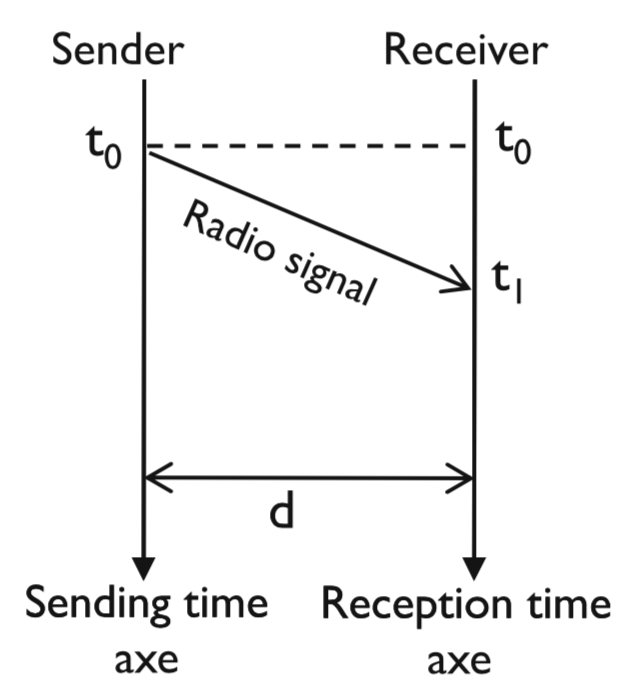
\includegraphics[width=.4\linewidth]{img/toa}
      \caption{Time of Arrival}
    \end{subfigure}%
    \begin{subfigure}{.5\textwidth}
      \centering
      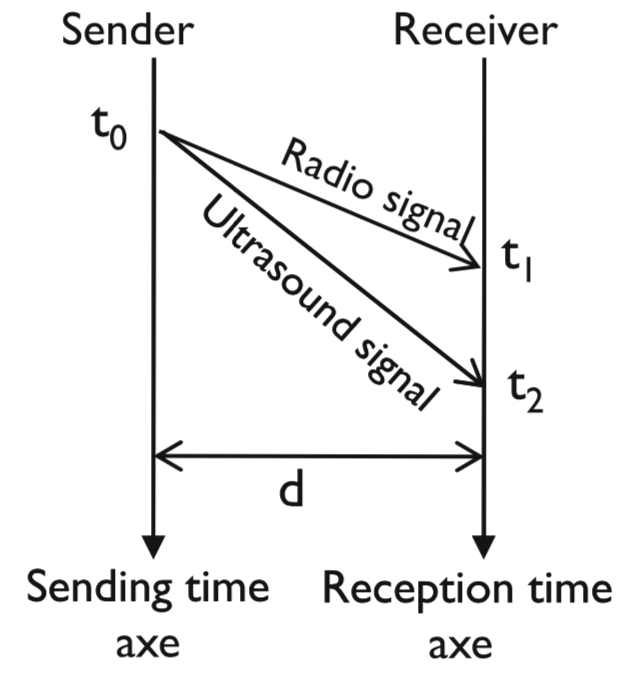
\includegraphics[width=.4\linewidth]{img/tdoa}
      \caption{Time Difference of Arrival}
    \end{subfigure}
    \caption{Time-based localization techiques}
    \end{figure}

    The TOA method can be used with Ultra-wideband (UWB) radio with which high accuracy can be achieved regardless the clock resolution thanks to the small propagation speed of ultrasound radios. This method is referred to as \textit{Time Difference of Arrival} (TDoA) and is based on the measurement of the time difference of the propagation of radio signals and ultrasound signals. When a node (anchor) simultaneously sends an RF signal and an ultrasound signal, the receiver (target) considers the arrival time of the (faster) radio signal as a time reference and uses the arrival time of the (slower) ultrasound radio to calculate the delay between the two signals. The distance is calculated according to Eq.~\ref{eq:tdoa}:

    \begin{equation}
    d = \frac{c_r \times c_u \times (t_2 - t_1)}{c_r - c_u}
    \label{eq:tdoa}
    \end{equation}

    where $c_r$ and $c_u$ are respectively the propagation speed of both radio and ultrasound signals, while $t_1$ and $t_2$ are their reception times at the receiver level.

    The TDOA method has the advantage to provide much better accuracy than RSS-based methods and it does not suffer from the need of explicit synchronization between nodes. However, it presents the drawback of requiring additional and more complex hardware with two different transceivers, which would have a negative impact on the cost.

    \item \textit{Angle of Arrival} relies on computing the angle by two lines connecting the unknown node with two anchor nodes. This technique relies on the use of directional antennas that can rotate on their axis or an array of antennas. For locating the unknown node at least three anchor nodes in 3D space and two anchor nodes in 2D space are needed.

    The advantage of AoA is that it does not require time sinchronization but on the other hand it requires vomplex and expensive hardware.
  \end{enumerate}

  \item \textbf{Estimation phase} (or combining distance): nodes use range information and anchors' locations to estimate their positions. In this phase some \textit{geometric geolocation techniques} are used:

  \begin{figure}[b]
    \centering
    \begin{subfigure}{.5\textwidth}
      \centering
      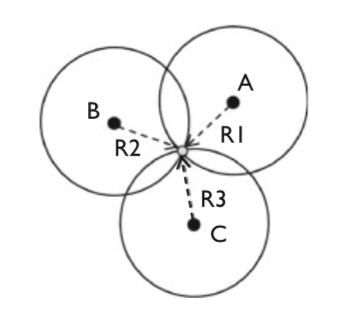
\includegraphics[width=.4\linewidth]{img/noise-free-lateration}
      \caption{with noise-free measurements}
    \end{subfigure}%
    \begin{subfigure}{.5\textwidth}
      \centering
      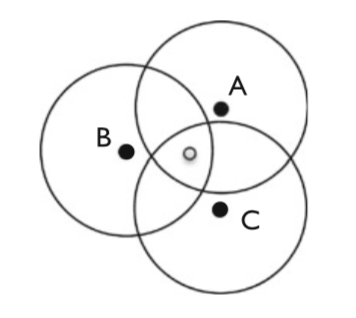
\includegraphics[width=.4\linewidth]{img/lateration}
      \caption{with noisy measurements}
    \end{subfigure}
    \caption{Trilateration technique}
  \end{figure}

  \begin{enumerate}[label=(\roman*)]
    \item \textit{Lateration/Trilateration} is the technique that uses distance information from anchor nodes to locate a target. In a 2D space, lateration involves the determination of the location of an unknown node as the intersection point of three circles centered in three non-collinear anchors (A, B and C), given that distances R1, R2 and R3 (i.e. circle radii) between the node and anchors are known. This technique is referred to as \textit{trilateration}. In a 3D space, there is a need of at least four anchor nodes to determine the location of a target node.
    \item \textit{Triangulation} is based on angle measurements to estimate the location of an unknown node.
    \item \textit{Multi-lateration} takes in consideration more than the minimum number of required anchor nodes.
  \end{enumerate}
\end{enumerate}

\paragraph{Limitations}
Some of the analyzed range-based localization techniques are based on assumptions that do not always hold or are impractical such as circular radio range, symmetric radio connectivity, lack of obstructions, clear line-of-sight.

\subsubsection{Range-free}
Range-free methods do not rely on distance or angle estimation in localization. They rather use proximity or connectivity information to devise the location of the target.

Anchor-based range-free localization techniques can be classified as:
\begin{enumerate}[label=(\alph*)]
  \item \textit{Area-based approaches} estimate the position of the target as a particular point in the polygon formed by the anchor nodes. Two main methods are proposed:
  \begin{enumerate}[label=(\roman*)]
    \item \textit{Centroid} consists in computing the location of the target as the \textit{centroid} point, defined as the barycenter of a set of anchors, as shown in Figure~\ref{fig:centroid}. In the most general form, assuming $n$ anchor nodes $A_i$ with coordinates $(X_i, Y_i )$ are detected by the target node (through beacon listening), the latter calculates its
    coordinate $(X_G, Y_G)$ such that:

    \begin{equation}
    (X_G, Y_G) = (\frac{\sum_{i=1}^n(X_i)}{n}, \frac{\sum_{i=1}^n(Y_i)}{n})
    \end{equation}

    Note that the more the number of anchors we have, the more accuracy we will obtain.

    \begin{figure}[t]
      \centering
      \begin{subfigure}{.5\textwidth}
        \centering
        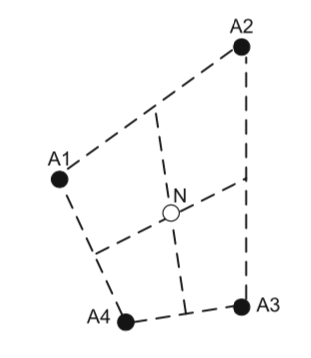
\includegraphics[width=.4\linewidth]{img/centroid}
        \caption{\label{fig:centroid}Centroid}
      \end{subfigure}%
      \begin{subfigure}{.5\textwidth}
        \centering
        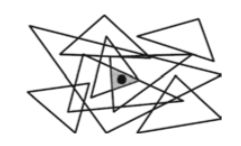
\includegraphics[width=.4\linewidth]{img/apit}
        \caption{\label{fig:apit}APIT}
      \end{subfigure}
      \caption{Area-base localization techniques}
    \end{figure}

    \item \textit{Approximate Point-In-Triangle (APIT)} assumes that the location of the target is the center of gravity of a certain triangle, which is defined as the intersection of triangles formed by anchors in which the target node resides, as illustrated in Figure~\ref{fig:apit}.

    The idea is to divide the environment into triangular regions, testing whether the target is inside a given triangle or not. The center of gravity of the triangles' intersection will represent the estimation target position.

    The main challenge in this technique is to determine whether the target is inside or outside a certain triangle. The idea, illustrated in Figure~\ref{fig:pit-test}, referred to as \textit{perfect PIT} and relies on checking the existence of a direction such that if the target moves according to that direction, it will simultaneously get further/closer to all triangle points, i.e. anchors.
    Two major handicaps hinder the practicability of this approach in real-world. First, nodes typically do not have the ability to recognize the direction without moving. Second, it is not possible to perform an exhaustive test covering all possible directions in which the target may move to. To solve both problems, an approximation has been proposed and whose idea is to use neighborhood information, exchanged via beaconing, to emulate the node movement in the Perfect PIT test as shown in Figure~\ref{fig:apit-test}:
    \begin{enumerate}[label=\arabic*.]
      \item The target node asks its neighbors for their distances to three corner anchors;
      \item The target compares its distance to these three corner anchors against those of its neighbors;
      \item If there exists at least one anchor such that it is further from or closer to all corner anchors than the target, then the latter considers itself as being outside the triangle.
    \end{enumerate}

    \begin{figure}[H]
      \centering
      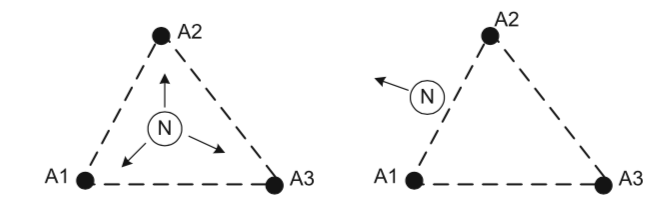
\includegraphics[width=0.7\textwidth]{img/pit-test}
      \caption{\label{fig:pit-test}Possible cases in point-in-triangle test. $N$ denotes the target node, and $A_i$ denotes the $i$-th anchor. The \textit{left figure} shows that if the target $N$ is inside the triangle moves in any direction, it will get close to some anchors and far from others. In the \textit{right figure}, if the target node $N$ is outside the triangle moves in the indicated direction, it will get far to all anchors at the same time.}
    \end{figure}

    \begin{figure}[h]
      \centering
      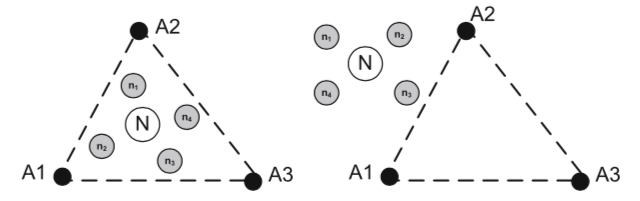
\includegraphics[width=0.7\textwidth]{img/apit-test}
      \caption{\label{fig:apit-test}Possible cases in approximate point-in-triangle test. $N$ denotes the target node, and $A_i$ denotes the $i$-th anchor. The \textit{left figure} shows that if the target $N$ is inside the triangle, none of its neighbors is either close to or far from all anchors. In the \textit{right figure}, if the target node $N$ is outside the triangle, its neighbor $n_1$ indicates that is it further to all anchors than it.}
    \end{figure}

   % TODO -- Relative Distance Estimation, Error scenarios, Pros and Cons

  \end{enumerate}
  \item \textit{Multi-hop localization approaches} are used when a target is not in communication range with at least three anchor nodes because of the limitation of the transmission power. In this case the idea consists in flooding the network such that each anchor independently broadcasts a \textit{beacon}, embedding its location and a hop-counter field initially set to one and increased in each new hop. Then, each target node identifies the shortest-path to each anchor node and tries to estimate its distance to it. One of the \textit{distance propagation methods} is:
  \begin{enumerate}[label=(\roman*)]
    \item \textit{DV-Hop}: the idea is to compute the number of hops between any two anchors $(A_i, A_j)$ and each anchor estimates the average 1-hop distance by dividing the sum of its distance to other anchors (\textit{physical distance}) by the sum of hop counts to those anchors (\textit{logical distance}). The process consists in three steps:
    \begin{enumerate}[label=\arabic*.]
    	\item \textit{Node update phase}: when a target node $N_i$ receives a beacon from an anchor, it maintains the record $(X_i, Y_i, h_i)$ for each anchor $A_i$, where $(X_i, Y_i)$ represents the location of the anchor, and $h_i$, the number of hops from $N_i$ to that anchor $A_i$.
    	\item \textit{1-hop distance estimation phase}: when an anchor node receives the locations and hop counts to the other anchors, it calculates the estimated average 1-hop distance, refereed to as \textit{correction factor} $c_i$, expressed as follows:
    	\begin{equation}
    	c_i = \frac{\sum(\sqrt{(x_i - x_j)^2 + (y_i - y_j)^2})}{\sum{(h_i)}}
    	\end{equation}
    	Then the anchor floods the network with the estimated 1-hop distance. A node that recives a correction, forwards it and then stops forwarding subsequent corrections.
    	\item \textit{Target node localization}: each target uses the correction sent from the \textbf{closest} anchor as the estimated 1-hop distance. It then multiplies the 1-hop distance by the hop counts to the other anchors to estimate its physical distance to them. After getting distance estimates to at least three anchors, a target can use trilateration to approximate its location.
    \end{enumerate}
    An example is shown in Figure~\ref{fig:dv-hop}.

    \begin{figure}[t]
      \centering
      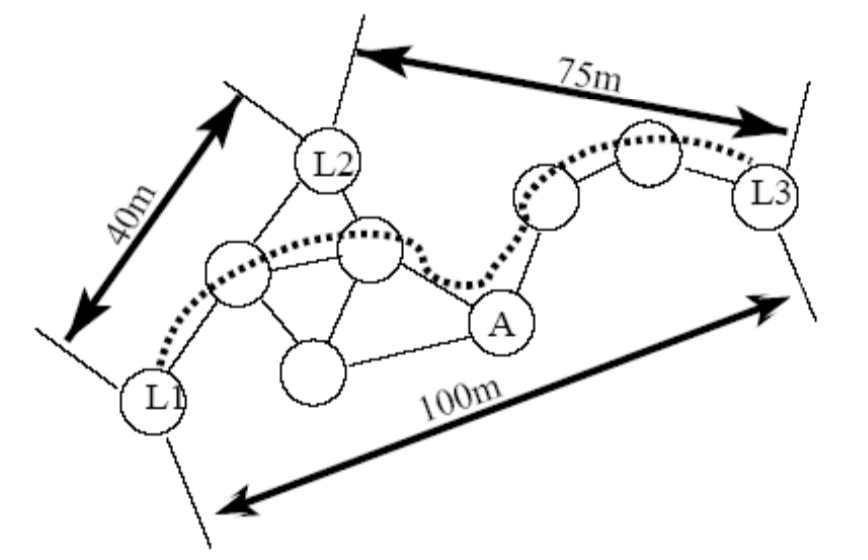
\includegraphics[width=0.4\textwidth]{img/dv-hop}
      \caption{\label{fig:dv-hop}DV-Hop example with anchor nodes $L_1$, $L_2$, $L_3$ and target node $A$. $c_1 = \frac{100+40}{6+2} = 17.5$, $c_2 = \frac{40+75}{2+5} = 16.42$, $c_3 = \frac{75+100}{6+5} = 15.90$. Target $A$ gets the correction from the closest anchor $L_2$ and computes the distance to $L_1 = 3 \times 16.42$, $L_2 = 2 \times 16.42$, $L_3 = 3 \times 16.42$.}
    \end{figure}
  \end{enumerate}
\end{enumerate}

\newpage

\section{Publish-Subscribe Pattern}
The Public-Subscribe pattern is a messaging pattern where sender of messages, called \textit{publishers}, do not program the messages to be sent directly to specific receivers, called \textit{subscribers}, but instead categorize published messages into classes without knowledge of which subscribers, if any, tehre may be.

Similarly, \textit{subscribers} express interest in one or more classes and only receive messages that are of interest, without knowledge of which publishers, if any, they are. The process of selecting messages for reception and processing is called \textbf{filtering}:
\begin{itemize}
  \item in a \textbf{topic-based} system messages are published to \textit{topics} and subscribers will receive only messages published to topics to which they subscribe.
  \item in a \textbf{content-based} system messages are only delivered to a subscriber if the attributes or content of those messages matches constraints defined by the subscriber.
\end{itemize}

Many solutions have been proposed for implementing the Publish-Subscribe system shown in Figure~\ref{fig:ps-problem}:
\begin{itemize}
  \item \textbf{client-server} solution is simple but not scalable, resulting in an overload on the server which is a single point of failure.
  \item \textbf{peer-to-peer (P2P)} architecture is a distributed system with a large number of heterogeneous and unreliable nodes, but it discloses the \textit{lookup} problem, i.e. how to know where the \textit{repository} node is. Three possible approach have been proposed:
  \begin{itemize}
    \item \textbf{centralized} approach based on a \textit{coordinator} node which must maintain $O(N)$ status and represents a single point of failure;
    \item \textbf{flooding} approach which foresees $O(N)$ messages per lookup;
    \item \textbf{DHT} approach which foresees $O(\log(N))$ messages per lookup, but building and maintenance of \textbf{routing tables} is needed.
  \end{itemize}
\end{itemize}

\begin{figure}[b!]
  \centering
  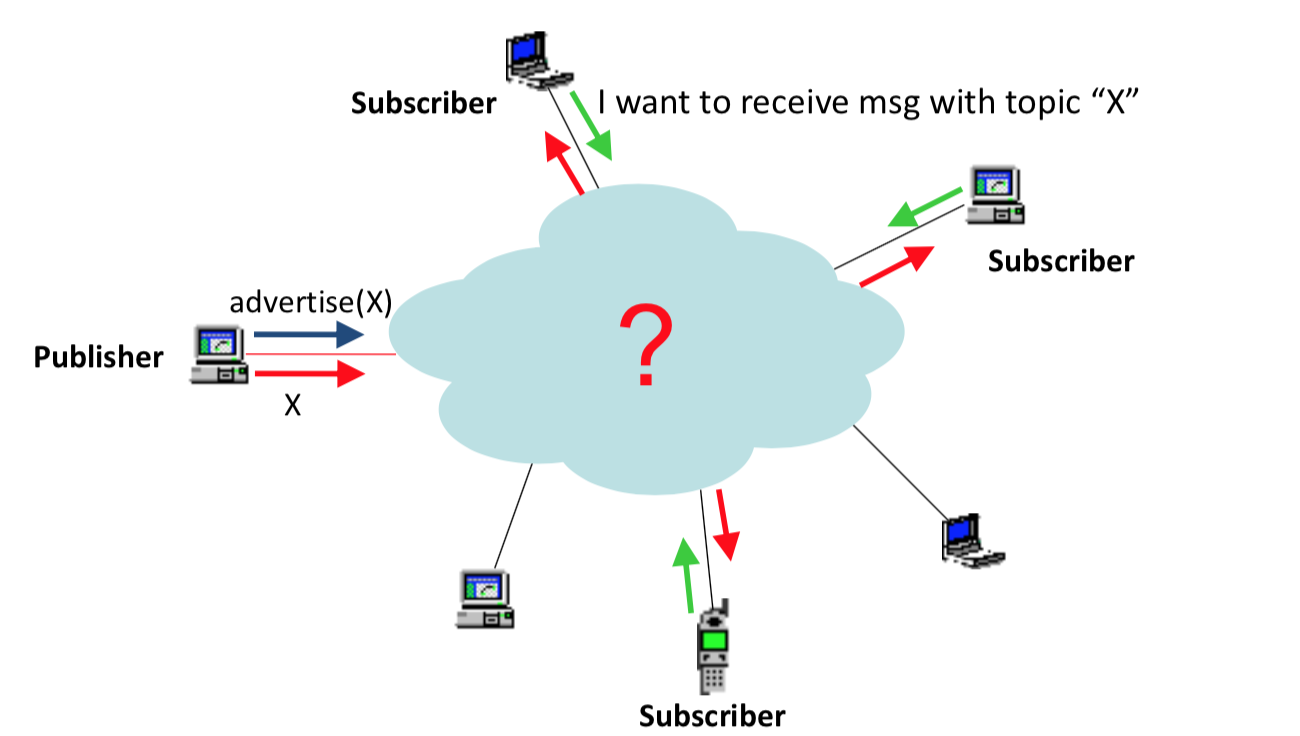
\includegraphics[width=0.8\textwidth]{img/ps-problem}
  \caption{\label{fig:ps-problem} Publish-Subscribe problem}
\end{figure}


\subsection{Distributed Hash Table (DHT)}
A Distributed Hash Table (DHT) described in Figure~\ref{fig:dht} is a distributed system that provides a \textbf{lookup} service similar to a hash table: $(key, value)$ pairs are stored in a DHT, and any participating node can efficiently retrieve the value associated with a given key. 

The main advantage of a DHT is that nodes can be added/removed with minimum work around re-distributing keys. Keys are unique identifiers which map to particular values, which in turn can be anything from addresses, to documents, to arbitrary data. Responsibility for maintaining the mapping from keys to values is distributed among the nodes, in such a way that a change in the set of participants causes a minimal amount of disruption. This allows a DHT to scale to extremely large numbers of nodes and to handle continual node arrivals, departures, and failures.

\begin{figure}[t]
  \centering
  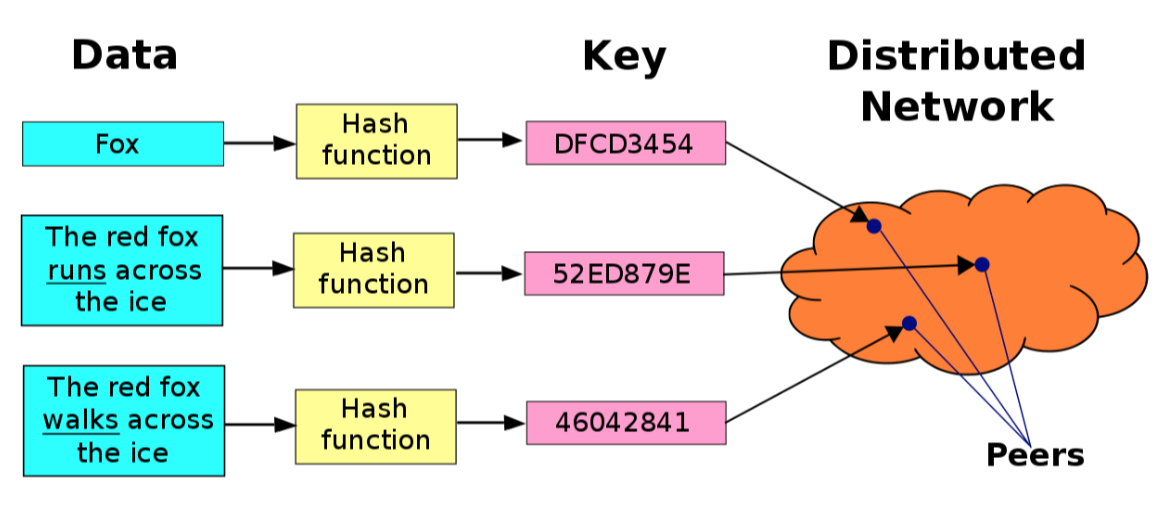
\includegraphics[width=0.7\textwidth]{img/dht}
  \caption{\label{fig:dht} DHT approach}
\end{figure}

\subsubsection{DHT structure}

The structure of a DHT can be decomposed into several main components:
\begin{itemize}
  \item an abstract \textbf{keyspace}, such as the set of 160-bit strings;
  \item a \textbf{keyspace partitioning scheme} splits ownership of this keyspace among the participating nodes;
  \item an \textbf{overlay network} then connects the nodes, allowing them to find the owner of any given key in the keyspace.
\end{itemize}

\begin{figure}[b!]
  \centering
  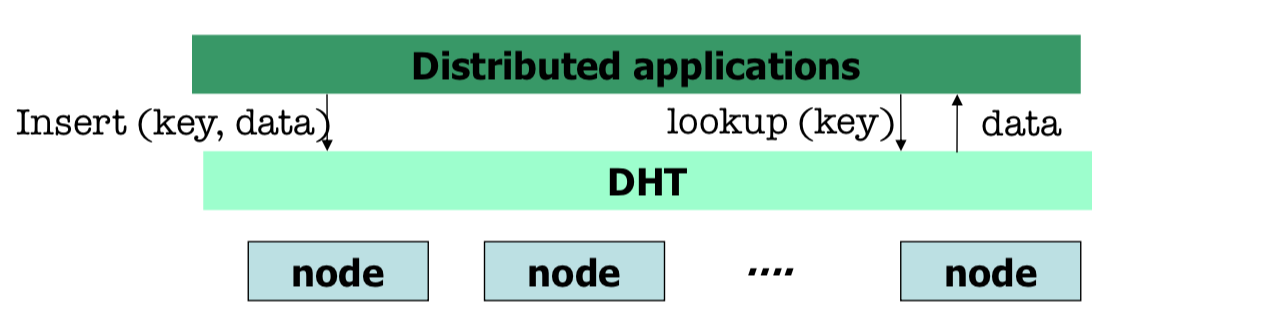
\includegraphics[width=0.8\textwidth]{img/dht-api}
  \caption{\label{fig:dht-api} DHT API}
\end{figure}

\subsubsection{DHT operations}

A typical use of the DHT for storage and retrieval might proceed as follows:
\begin{enumerate}[label=\arabic*.]
  \item to index a file with given filename and data in the DHT, the SHA-1 hash of filename is generated, producing a 160-bit key $k$, and a message \texttt{insert(k, data)} is sent to a node participating in the DHT.
  \item the message is forwarded from node to node through the overlay network until it reaches the single node responsible for key $k$ as specified by the keyspace partitioning. That node then stores the key and the data.
  \item any other client can then retrieve the contents of the file by again hashing filename to produce $k$ and asking a DHT node to find the data associated with $k$ with a message \texttt{lookup(k)}.
  \item the message will again be routed through the overlay to the node responsible for $k$, which will reply with the stored data.
\end{enumerate}

\subsubsection{DHT properties}

DHTs characteristically emphasize the following properties:
\begin{itemize}
  \item \textit{Autonomy and decentralization}: the nodes collectively form the system without any central coordination.
  \item \textit{Fault tolerance}: the system should be reliable even with nodes continuously joining, leaving, and failing.
  \item \textit{Scalability}: the system should function efficiently even with thousands or millions of nodes.
  \item \textit{Load Balancing}: the hash function should evenly distribute keys to nodes.
  \item \textit{Anonimity}: can be achieved by special routing overlay networks that hide the physical location of each node from other participants.
\end{itemize}

\subsection{Pastry}

\subsection{Scribe}







\end{document}